\documentclass[journal]{IEEEtran}

% *** CITATION PACKAGES ***
%
%\usepackage{cite}
\usepackage{capt-of}%%To get the caption
\usepackage{gensymb}
\usepackage{graphicx} %package to manage images
\graphicspath{ {./images/} }
\usepackage{wrapfig}
\usepackage{xcolor}


\usepackage{amsmath}
\usepackage{amssymb}

\usepackage{lipsum}

\usepackage[style=ieee]{biblatex}
\DeclareLanguageMapping{english}{english-apa}
\addbibresource{references.bib}
\usepackage[justification=centering]{caption}

\usepackage{setspace}

\usepackage{hhline}


\usepackage{changepage} 

\usepackage{booktabs}
\usepackage{xcolor}

\usepackage{makecell}
\usepackage{graphicx,subcaption}
\usepackage{listings}
\renewcommand\theadfont{}
\DeclareMathOperator{\EX}{\mathbb{E}}% expected value
\newcommand{\cc}[1]{\texttt{#1}}


\usepackage{multicol} 

\raggedbottom

\begin{document}


\pagenumbering{gobble}
%\clearpage\mbox{} % adds and empty page
%\clearpage
\pagenumbering{arabic}
\setcounter{page}{1}

\title{{\large Mini Project 3: Predicting Ridership and Hottest Pickup Zones in January Based on Weather Data}}

\author{ENGR-UH 4560 Machine Learning, Fall 2019\\
\medskip
Barkin Simsek,~\IEEEmembership{bs3528@nyu.edu};
Nishant Aswani,~\IEEEmembership{nsa325@nyu.edu}}% <-this % stops a space


% The paper headers
\markboth{Simsek, Aswani, ENGR-UH 4560 Selected Topics in  Information and Computational Systems Machine Learning, Fall 2019}%
{}

% make the title area
\maketitle

% As a general rule, do not put math, special symbols or citations
% in the abstract or keywords.
\begin{abstract}
for the airplane
\end{abstract}

%%%%%%%%%%%%%%%%%%
%% Introduction %%
%%%%%%%%%%%%%%%%%%
\section{Introduction}
\subsection{Research Motivation}
{\color{blue} for the airplane}

\subsection{Research Objective}
{\color{blue} for the airplane}

\subsection{Scoping the Project}
\noindent Having plotted the pickup location heatmap, we decided to limit our exploration to Manhattan. Figure \ref{fig:heatmap}, plotted with a random subset of data, shows Manhattan to have the hottest pickup locations. Although not visible below, another popular pickup area is the airports. However, given our focus on weather's effects, we deemed it was appropriate to leave airports out, as taxi pickups are most likely independent of weather conditions.\\

\begingroup
    \centering
    %width=\columnwidth
    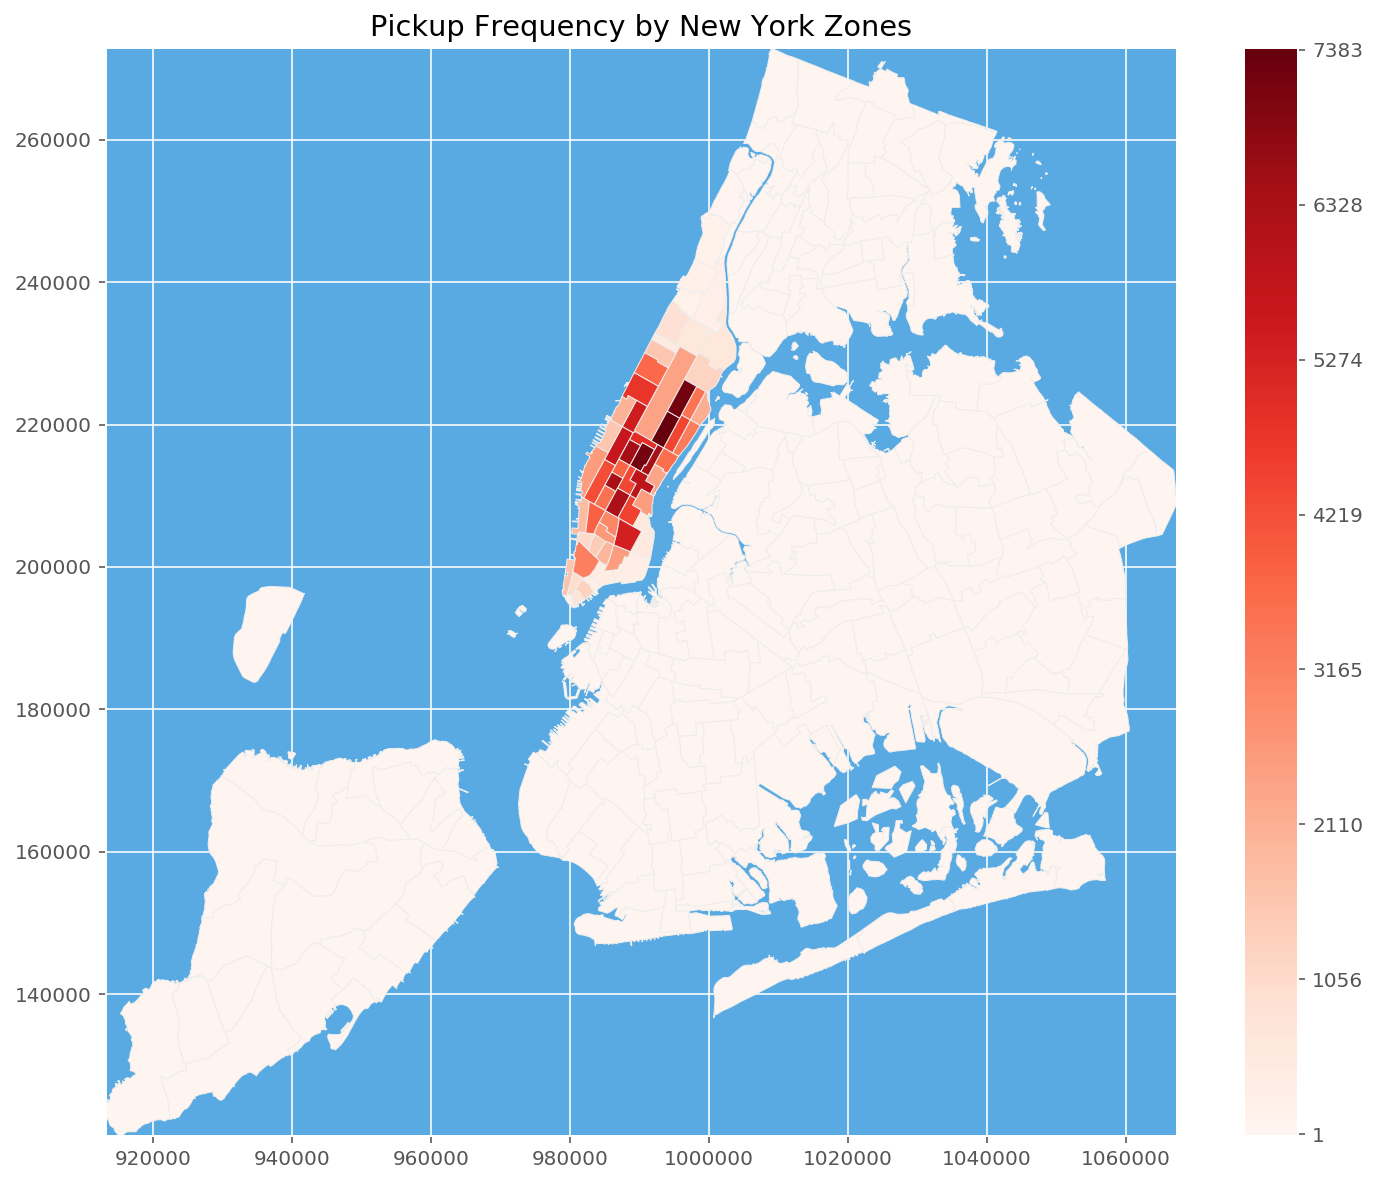
\includegraphics[width=\columnwidth]{images/heatmap.png}
    \captionof{figure}{Pickup frequency by zones}
    \label{fig:heatmap}
    \medskip
\endgroup

\noindent We chose to pursue this idea after visualizing the timeseries pattern of precipitation against the pickup counts. Figures \ref{fig:2017_rain_count} and \ref{fig:2018_rain_count} show promising correlations between ridership and precipitation on days of extreme weather conditions.

\begingroup
    \centering
    %width=\columnwidth
    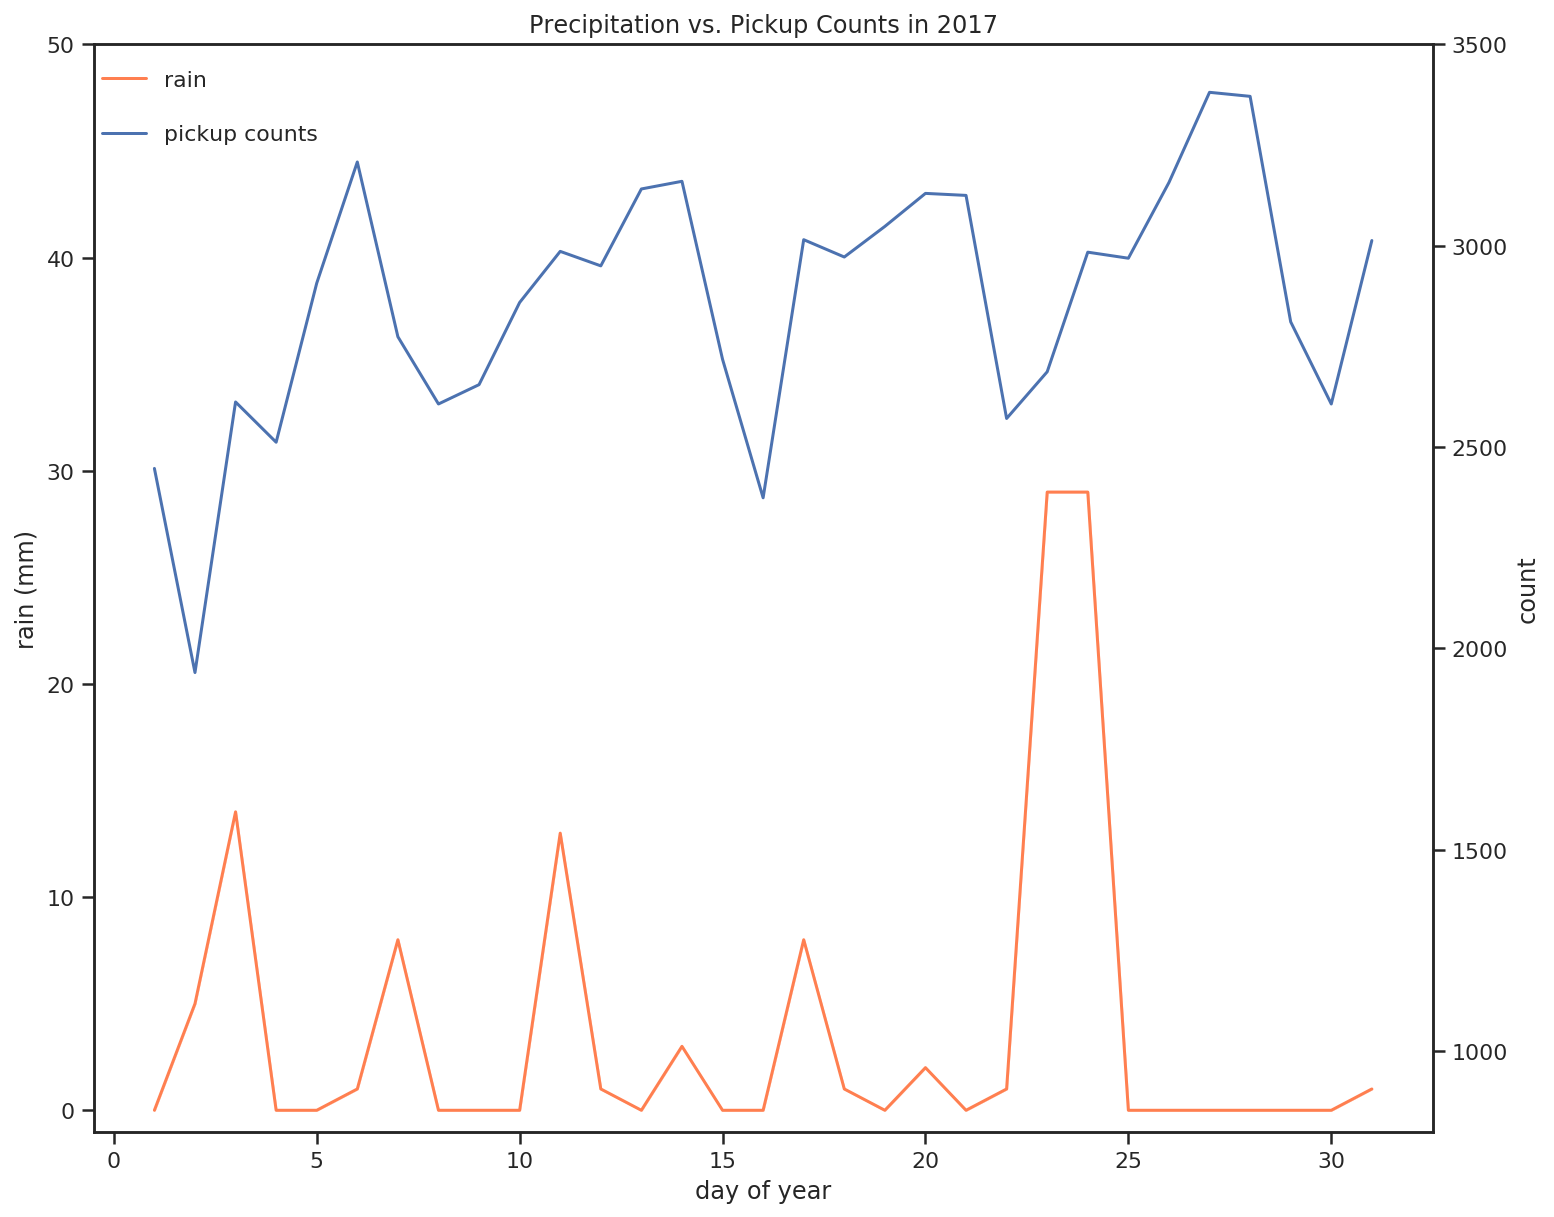
\includegraphics[width=\columnwidth]{report/images/2017_rain_count.png}
    \captionof{figure}{Precipitation vs. pickup counts in 2017}
    \label{fig:2017_rain_count}
    \medskip
\endgroup
\begingroup
    \centering
    %width=\columnwidth
    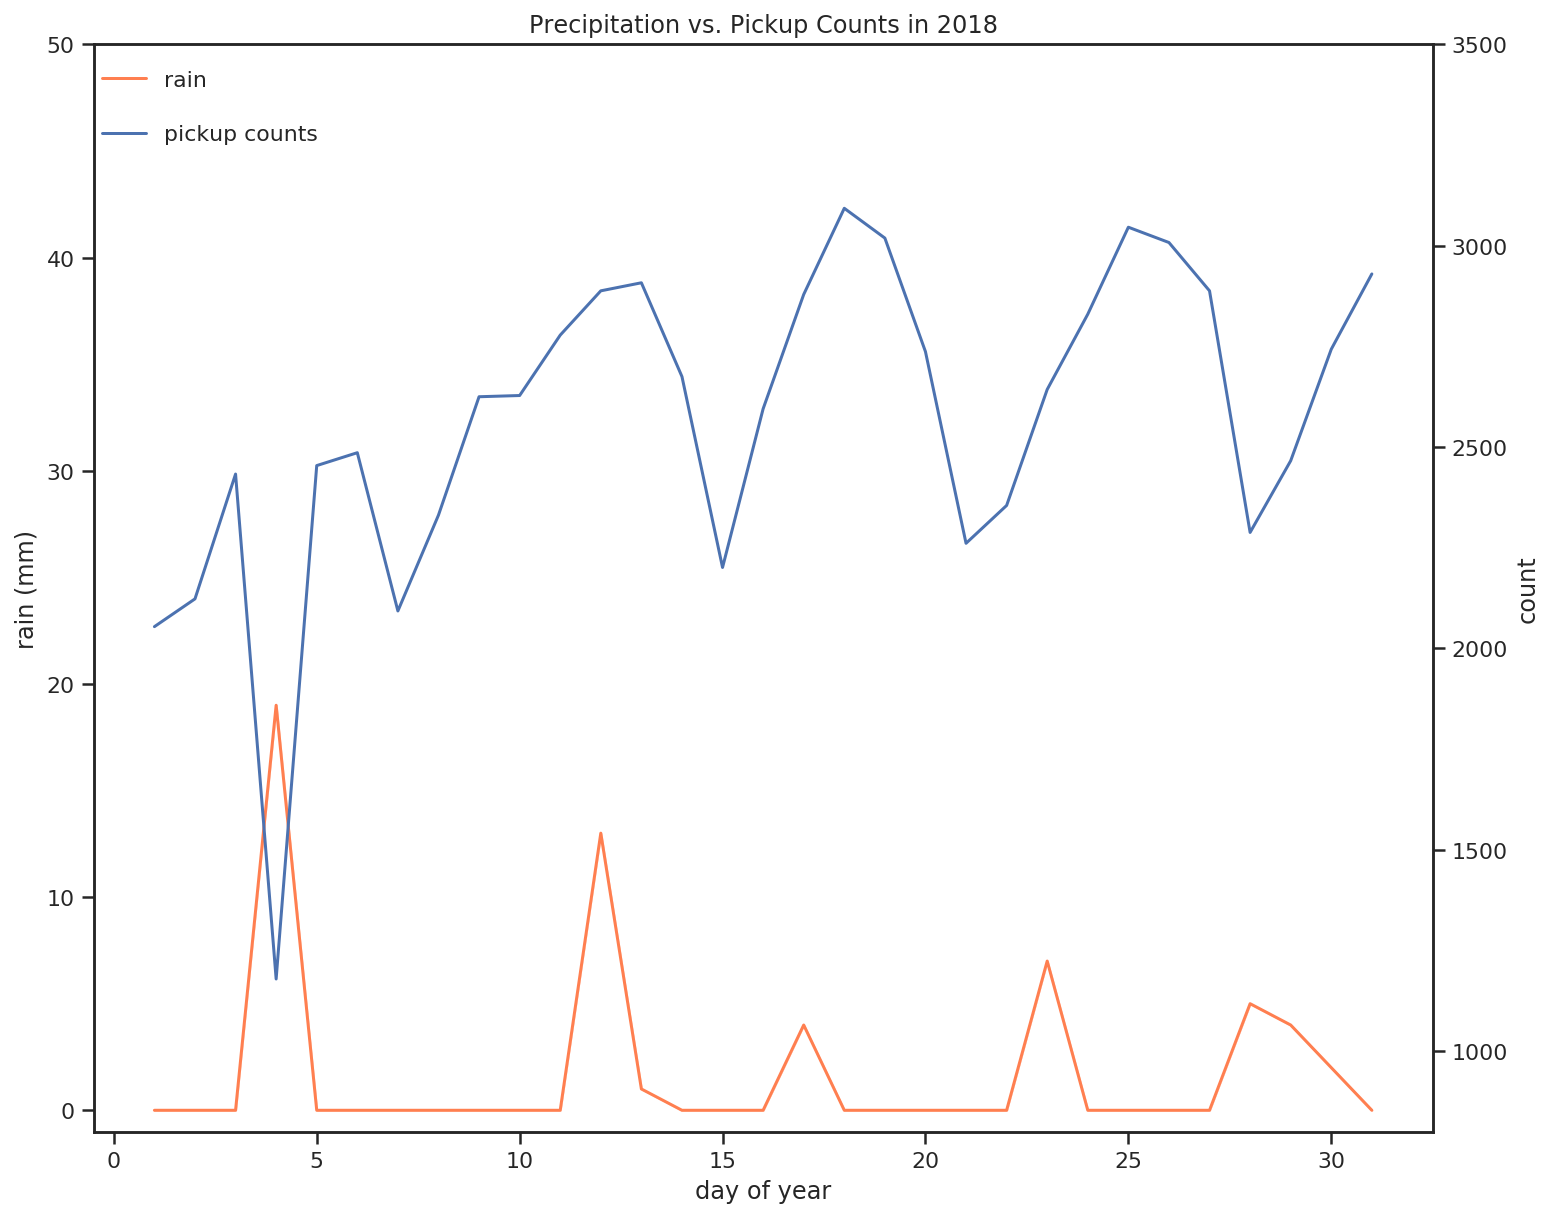
\includegraphics[width=\columnwidth]{report/images/2018_rain_count.png}
    \captionof{figure}{Precipitation vs. pickup counts in 2018}
    \label{fig:2018_rain_count}
    \medskip
\endgroup


%%%%%%%%%%%%%%%%%%%%%%%%%%%%%%%%%%%
%% Data Processing and Filtering %%
%%%%%%%%%%%%%%%%%%%%%%%%%%%%%%%%%%%
\section{Data Procurement, Processing, and Filtering}

\noindent Data was loaded into the workspace using the dask dataframe allowing for quicker access. As part of the \cc{read\_csv} function, the  \cc{tpep\_pickup\_datetime} and \cc{tpep\_dropoff\_datetime} columns were parsed as datetime formatted to allow for easier indexing and future data cleaning. Upon reviewing the dataframe, there were $1.846966e+07$ data points for 2017 and 2018 January. The challenge was then to identify methods for removing worthless datapoints and selecting a subset for training and testing. We decided against using the entire dataset because of limited computational resources. 

\subsection{Checking for Anomalies in TLC Data}

\noindent Once it was confirmed that there were no null values present in the 2017 and 2018 January dataset, we selected a {\color{red} 1\% fraction} of the dataset to build our code with. We then sorted and reindexed the data to obtain a dataframe of purely January datapoints, removing stray datapoints from different months or years.\\

\noindent To aid in finding unreasonable data, we turned to the Adopted Rules of the Taxi and Limousine Comission (TLC). The maximum trip duration is 12 hours. Hence, we iterated through all columns to determine the trip duration by subtracting pickup time from dropoff time. Any duration greater than 12 hours {\color{blue} or in negative time} was deemed to be garbage and was removed from the dataset. In each iteration we also calculated the speed and removed all results with values less than 0 or greater than 90. Whiel\\

\noindent For the remaining columns, such as \cc{total\_amount} and \cc{extra}, all rows with values less than zero were removed. 

\subsection{Shapefile Data}

\noindent Having little experience with shapefiles, we relied on functions from an existing machine learning project \cite{shapefile} to manipualate the shapefile and produce maps with a pick up heatmap. 

\subsection{Weather Data}

\noindent Despite being relatively simple data, we ran into some trouble obtaining weather data for New York. As we had decided to focus on Manhattan, we found it fit to select a weather station there and select data between 2017 and 2018.\\

\noindent {\color{blue} Add details about obtaining data}\\

\noindent Examining our dataset, we found null values for some days. Instead of removing them, we made the decision to linearly interpolate the data so as not to render corresponding values in our taxi dataframe unusable. Next, we combined the date, month, and year columns to produce a datetime column. In order to correspond the weather data with the TLC data, we used the \cc{pd.to\_datetime} method to obtain an indexable column. Using this column, we then merged  the relevant rain, average temperature, and average humidity data into the main dataframe.

%%%%%%%%%%%%%%%%%
%% Methodology %%
%%%%%%%%%%%%%%%%%
\section{Methodology}

\subsection{Data Visualization}

\noindent After meticulous cleaning and data vetting, we produced a dataframe combining taxi and weather data named \cc{nyc\_df}. We used this data to visualize the relation between ridership and the three weather features. Figures \ref{fig:2017_rain_count}, \ref{fig:2018_rain_count}, and the following figures allow for a rough visualization of any timeseries correlations. 

\begingroup
    \centering
    %width=\columnwidth
    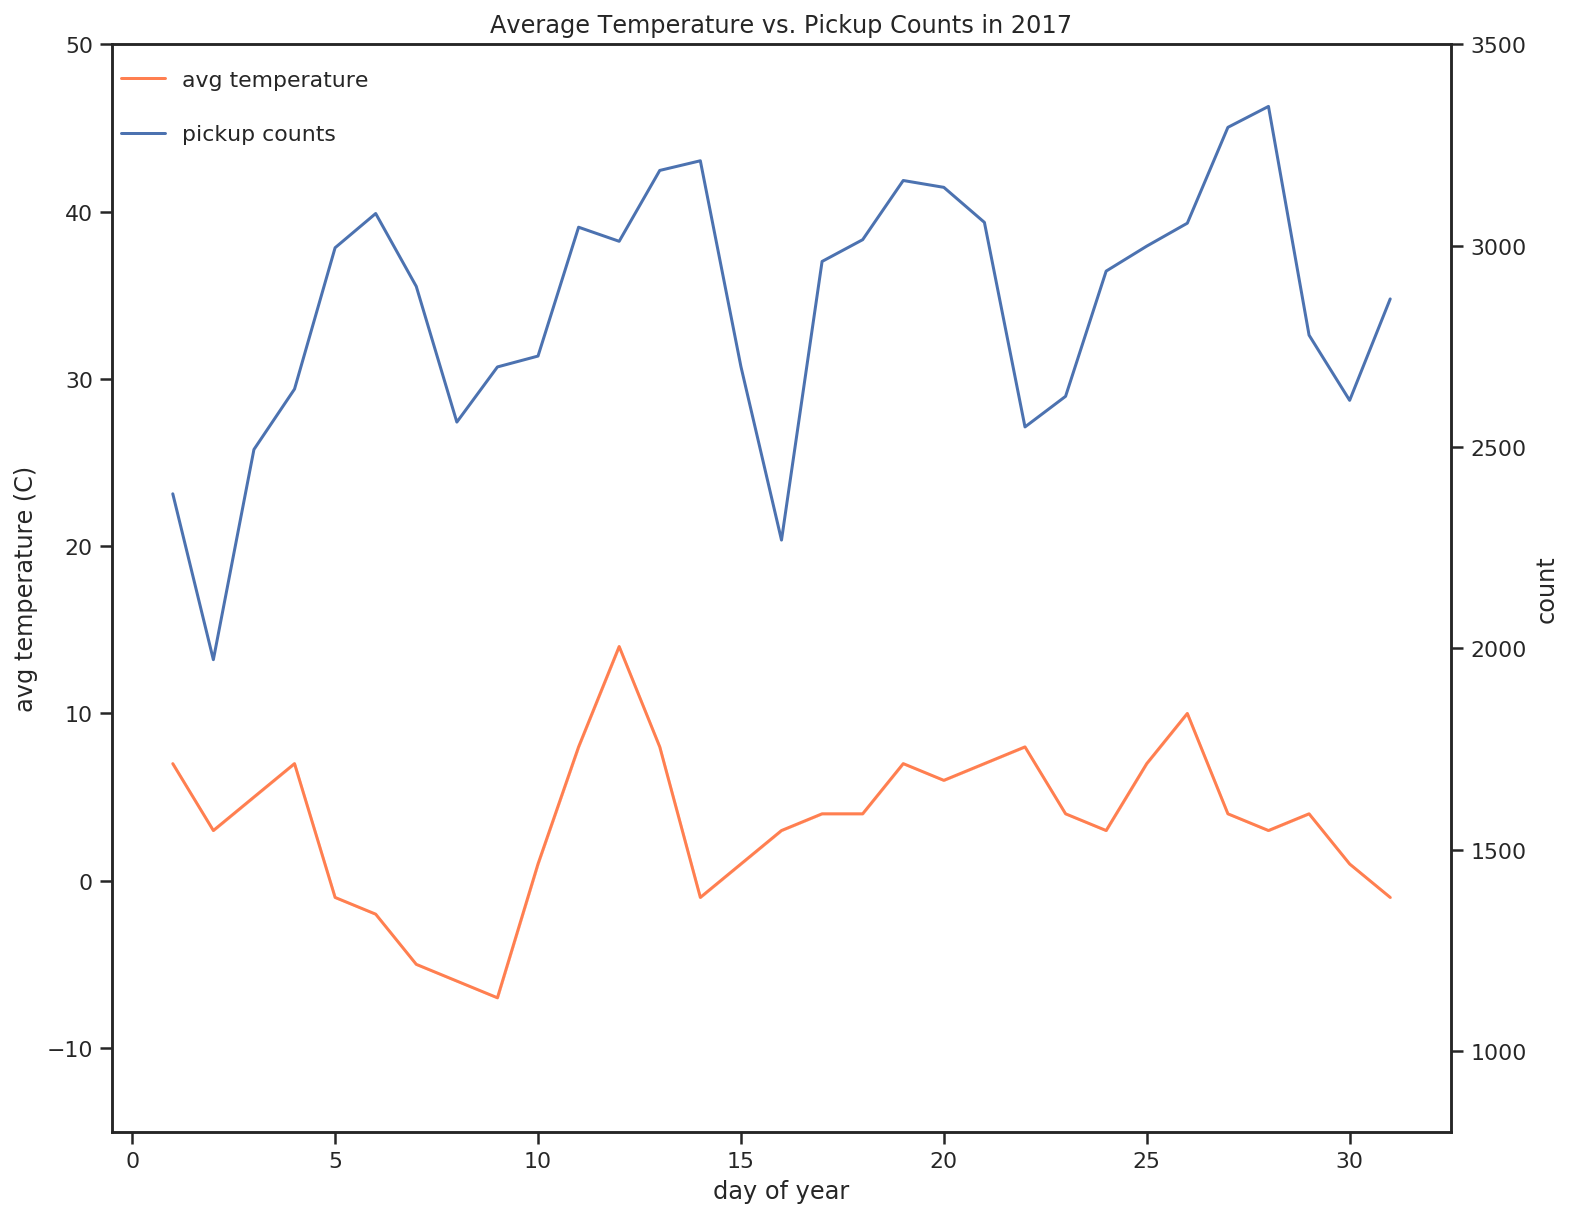
\includegraphics[width=\columnwidth]{report/images/2017_temp_count.png}
    \captionof{figure}{Average temperature vs. pickup counts in 2017}
    \label{fig:2017_temp_count}
    \medskip
\endgroup
\begingroup
    \centering
    %width=\columnwidth
    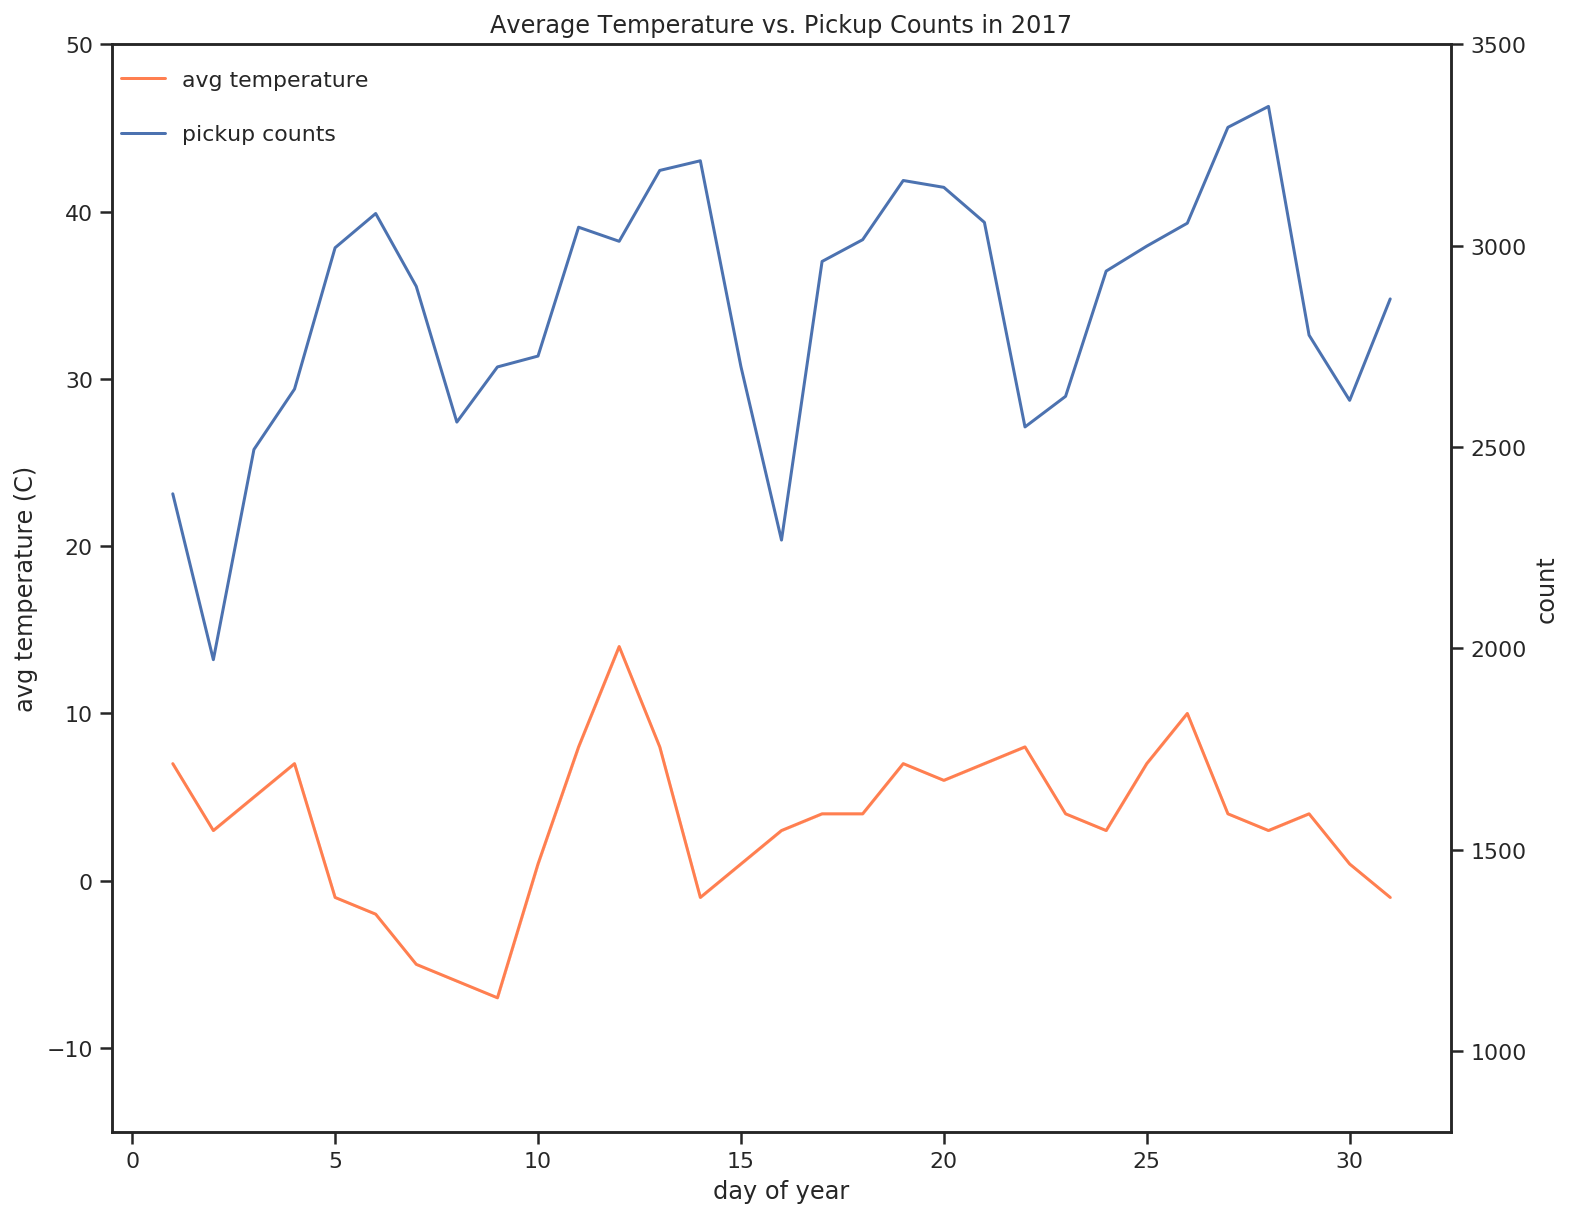
\includegraphics[width=\columnwidth]{report/images/2017_temp_count.png}
    \captionof{figure}{Average temperature vs. pickup counts in 2018}
    \label{fig:2018_temp_count}
    \medskip
\endgroup

\begingroup
    \centering
    %width=\columnwidth
    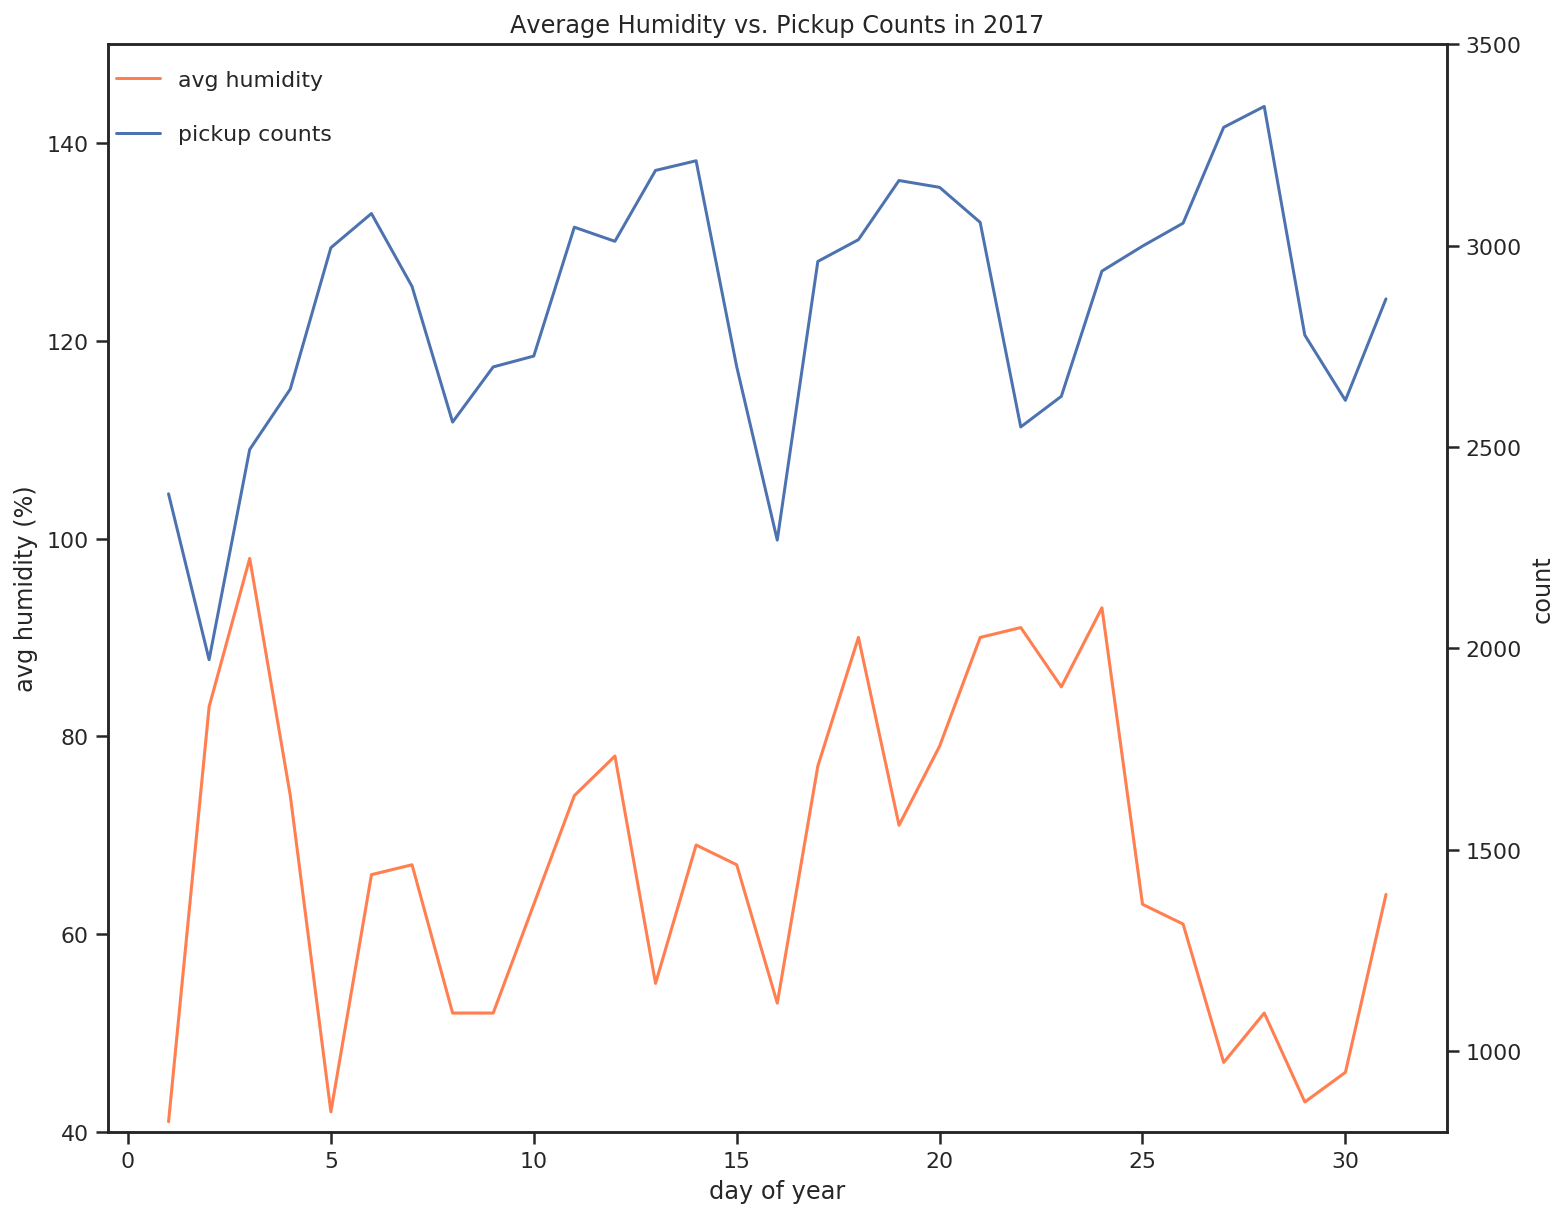
\includegraphics[width=\columnwidth]{report/images/2017_humidity_count.png}
    \captionof{figure}{Average humidity vs. pickup counts in 2017}
    \label{fig:2017_hum_count}
    \medskip
\endgroup
\begingroup
    \centering
    %width=\columnwidth
    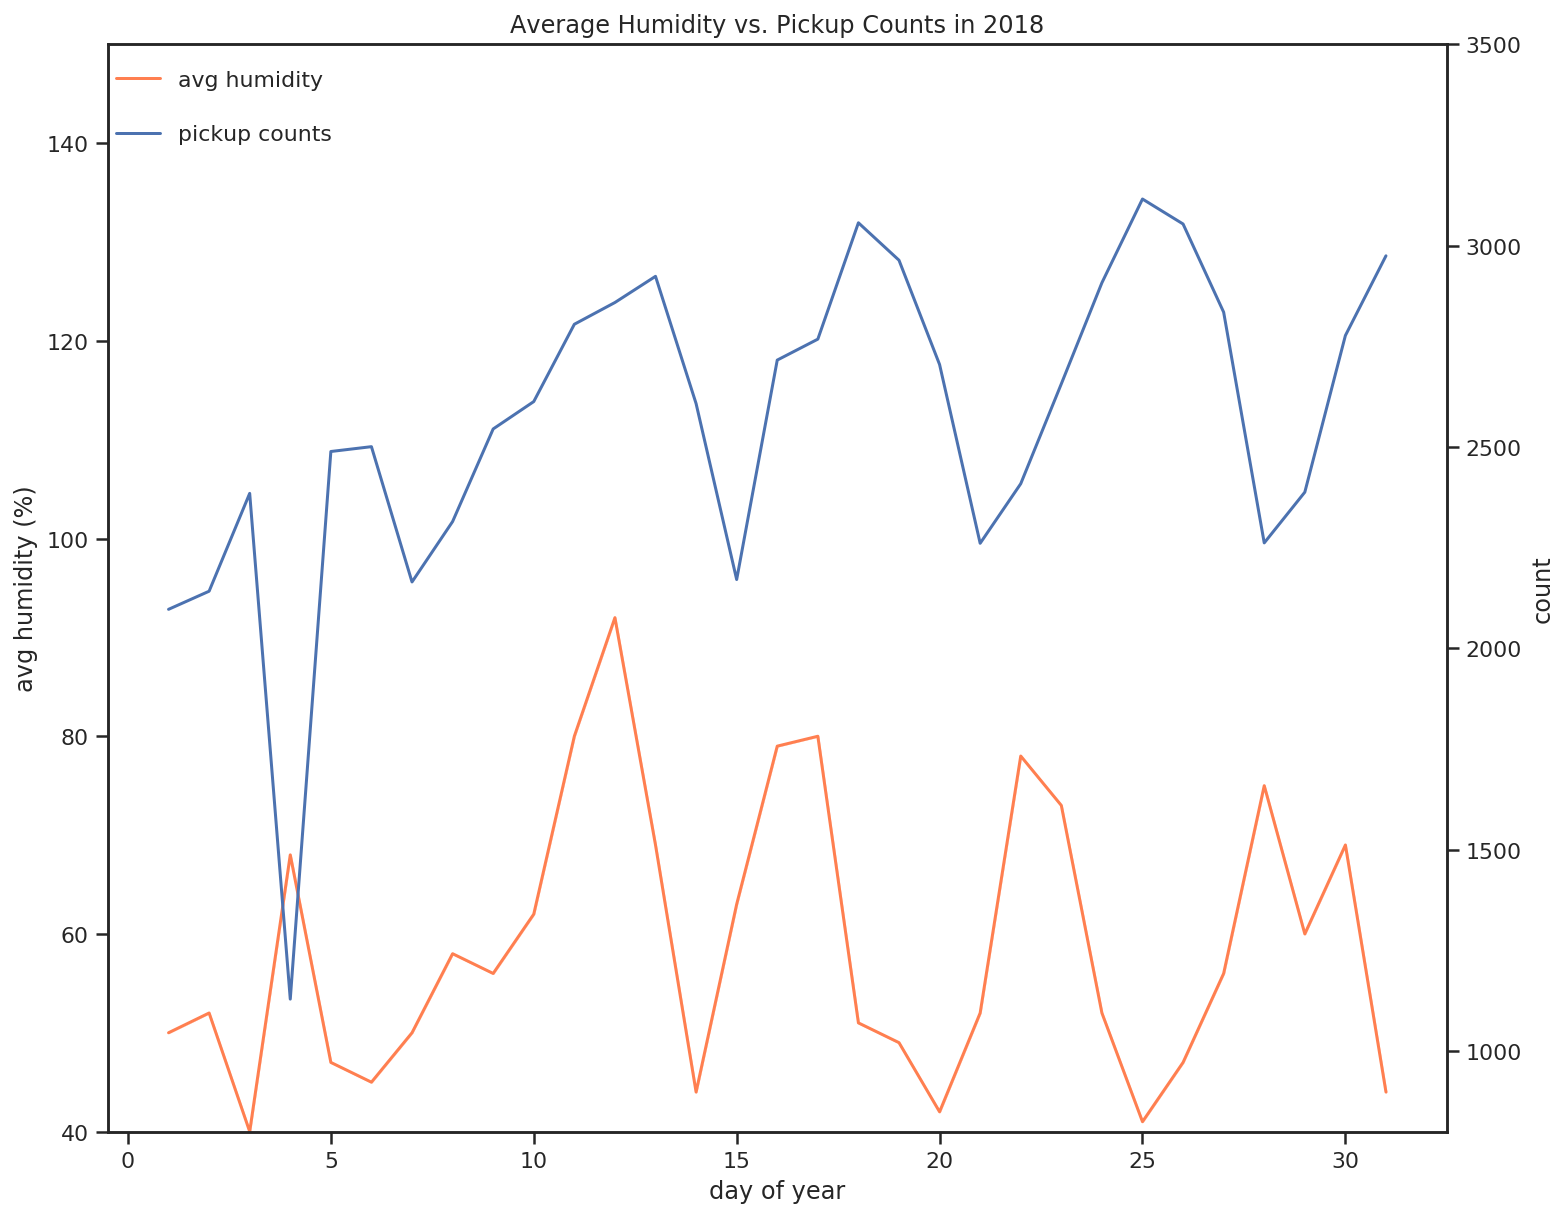
\includegraphics[width=\columnwidth]{report/images/2018_humidity_count.png}
    \captionof{figure}{Average humidity vs. pickup counts in 2018}
    \label{fig:2018_hum_count}
    \medskip
\endgroup

\subsection{Training Preparation}

\noindent After obtaining these timeseries visualizations we were adamant to move forward with the project, as the data seemed to suggest that extreme weather events affected ridership. For example, days with high humidity and precipitation tend to reduce ridership. This insight, combined with the inference that extreme weather reduces taxi mobility, implies that it becomes more imperative for.\\

\noindent We used \cc{nyc\_df} to produce \cc{df\_17} and \cc{df\_18}, both of which contain the day of the month, locationID, rainfall, average temperature, average humidity, and pickup count, for the years 2017 and 2018, respectively. Figure \ref{fig:train_test_df} shows how the dataframes look. \\

\begingroup
    \centering
    %width=\columnwidth
    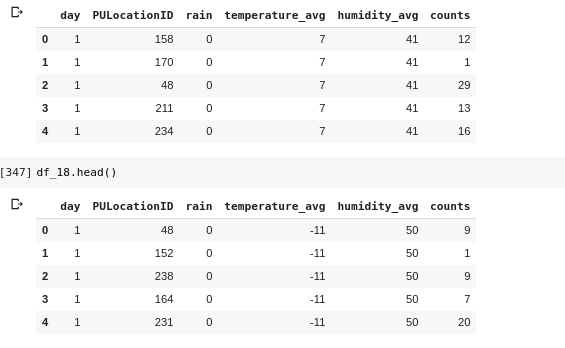
\includegraphics[width=\columnwidth]{report/images/train_test_df.png}
    \captionof{figure}{Snippets of df\_2017 and df\_2018}
    \label{fig:train_test_df}
    \medskip
\endgroup

\noindent Instead of the traditional \cc{train\_test\_split} method, we opted to make 2017 the training data and 2018 the testing data. This allows for us to test how well our model performs given how an entire month looks like. If this were to be used as an application or software, this implementation would make the most sense, as the user would simply input the aggregate data of the current year.

\subsection{Linear Regression}

\noindent Linear regression makes the assumption that there is a linear correlation between the independent and dependent variable. While this may seem easily dismissable, it is interesting to dissect this model. Looking at the data visualizations in the sections above, we noticed that on heavy weather event days, there was lower ridership. Hence, it may not be completely absurd to apply a linear fit to the model. However, because we also include day of the month and location ID as features, it becomes less reasonable to use a linear regression model.\\

\noindent For this implementation we simply used the \cc{squared\_loss} as the loss function and applied a grid search over a range of alpha values, optimizing for negative mean absolute error with 3-cross-fold validation. We then calculated the \cc{mean\_absolute\_errors} and \cc{mean\squared\_errors} for the training and test fits. \\

\subsection{Random Forest Regression}

\noindent Random forest regression operates on the idea of multiple decision trees. Each of these trees is built by randomly selecting data (with replacement) to create a bootstrapped dataset \cite{randomforest}. Randomly selected features from the bootstrapped dataset are then used to decide what the root node for the decision tree is. This process is repeated multiple times to obtain a "forest". The data is then used to run down each of the trees and obtain the final answer.\\

\noindent For our experiment we searched through\cc{[10, 40, 80, 160, 320]} to find the optimal number of trees in the forest, seeking to minimize the negative mean absolute error and using 3 folds cross validation. We then trained a model with this and obtained the \cc{mean\_absolute\_errors} and \cc{mean\squared\_errors} for the training and test fits along with the accuracy. We also sought the out of bag error, which simply tests datapoints on trees that did not use those datapoints to build their bootstrap dataset for a score. Moreover, we also extracted the feature importances to view how important weather data was for our experiment when compared with day and location ID. \\

\subsection{XGBoost Regression}

\noindent XGBoost Regression is built upon the idea of decision trees, but it incorporates the errors of previous trees to build better ones in the future. Our XGBoost model takes the average of all pick up counts. The next tree built simply takes the errors into account by subtracting the calculated pick up average by the actual amount for each datapoint. However, the depth of each tree is specified. In each tree, each residual is added to the sum to obtain a guess. However, the XGBoost Regressor model avoids the high variance problem (overfitting problem) by assigning a learning rate to each of the trees so only small steps are taken in (hopefully) the right direction.\\

\noindent For our model, we searched through [4, 8, 10, 15, 20, 25, 32] as options for depth and [40, 80, 150, 600] as options for number of trees, minimizing for squared error and using 3 folds cross validation. We then obtained the the \cc{mean\_absolute\_errors} and \cc{mean\squared\_errors}, as well as the accuracy scores to test for performance. 

\subsection{KNeighbors Regression}

\noindent We also used the K Nearest Neighbors Regressor to predict the pickup count. The idea of KNR significantly deviates from decision trees, because KNR makes its decisions based on how close another datapoint is numerically. At first thought, this may seem to work because the algorithm would likely correlate location ID and give counts based on how close it is to another location. However, looking at the location file, we see that the IDs are not assigned based geographically. In other words, location 1 is not necessarily geographically close to location 2. 

\subsection{Expectations}

\noindent From the analyses above, we did not expect promising results from the linear and KN regression models because of their assumptions. We did expect reasonable results from the decision-tree-based models because of their approach. 

%%%%%%%%%%%%%
%% Results %%
%%%%%%%%%%%%%
\section{Initial Results}

\noindent Below, MAPE refers to mean absolute percentage error and MSE refers to the mean squared error.

\subsection{Linear Regression}

\noindent GridSearchCV selected alpha = 130 and produced the following results\\

\begingroup
    \medskip
    \centering
    \def\arraystretch{1.5}
        \begin{tabular}{ccccc}
            \toprule
            TrainMAPE & TrainMSE & TestMAPE & TestMSE & R^2 \\
            \midrule
            70.58 & 591878 & 75.31 & 528067 & -0.014\\
            \bottomrule
        \end{tabular}
    \captionof{table}{Linear regression results}
    \label{table:}
    \medskip
\endgroup

\subsection{Random Forest Regression} 

\noindent GridSearchCV initially selected for 320 trees. The range of tree selection was then updated to   values = [320, 350, 400, 500, 600, 700, 800, 900], from which it selected 400 trees. Although, this value did not remain consisten after multiple runs.\\

\begingroup
    \medskip
    \centering
    \def\arraystretch{1.5}
        \begin{tabular}{ccccc}
            \toprule
            TrainMAPE & TrainMSE & TestMAPE & TestMSE\\
            \midrule
            27.94 & 95001 & 77.89 & 585321\\
            \bottomrule
        \end{tabular}
    \captionof{table}{Random Forest regression results}
    \label{table:}
    \medskip
\endgroup

\begingroup
    \medskip
    \centering
    \def\arraystretch{1.5}
        \begin{tabular}{ccc}
            \toprule
            Train Score & Test Score & OOB Score\\
            \midrule
            0.84 & -0.12 & -0.1929\\
            \bottomrule
        \end{tabular}
    \captionof{table}{Random Forest regression results}
    \label{table:fifty_runs}
    \medskip
\endgroup

\noindent We also plotted the feature importances for the random forest to see how the regression model weighted each feature. We learned that the model weighed LocationID as the most important feature, followed by day, humidity, temperature.\\

\begingroup
    \centering
    %width=\columnwidth
    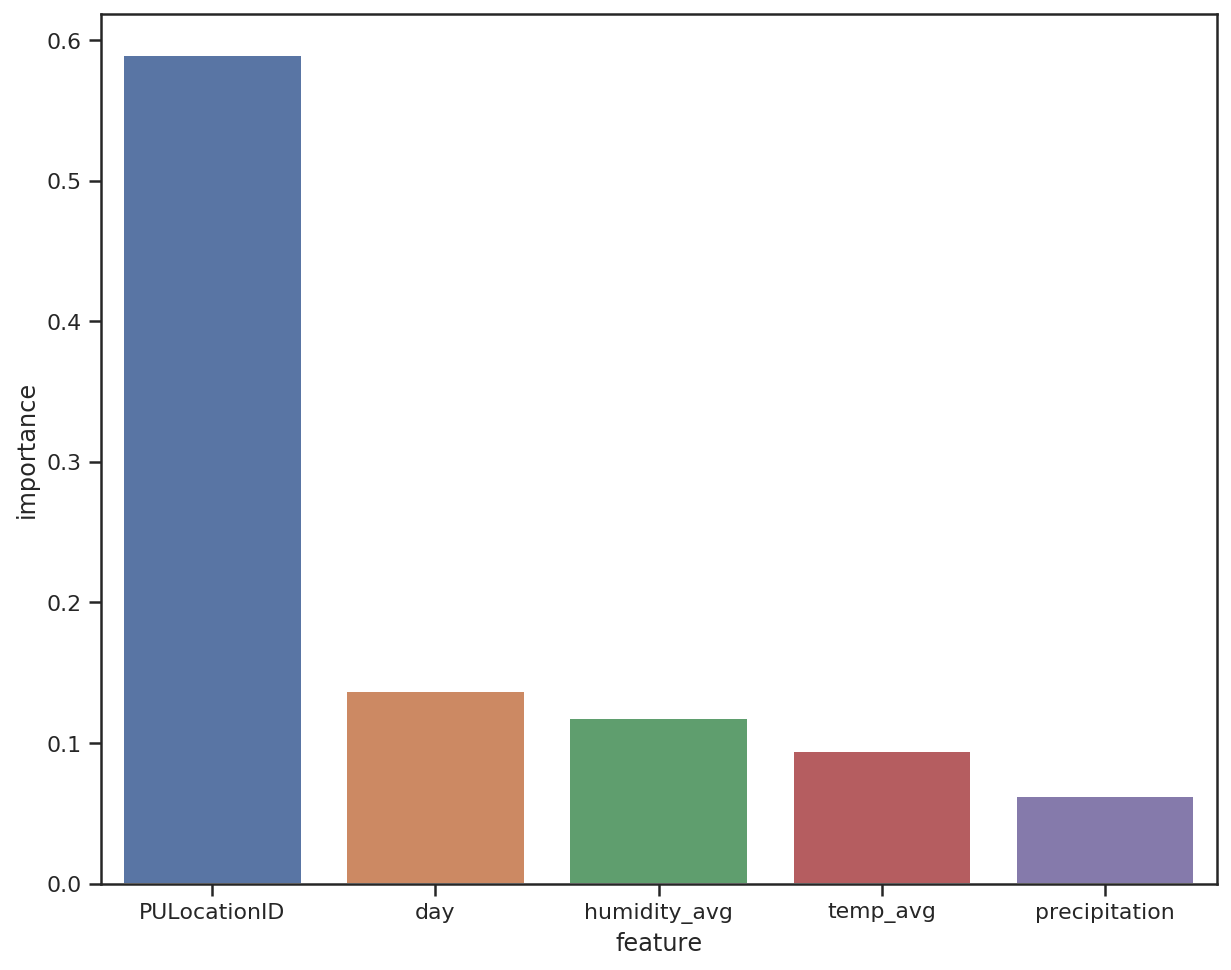
\includegraphics[width=\columnwidth]{report/images/feature_importance_rf.png}
    \captionof{figure}{Feature importance in Random Forest Model}
    \label{fig:train_test_df}
    \medskip
\endgroup

\subsection{XGBoost Regression}

\noindent XGBoost selected for 40 estimators with a tree depth of 1.\\

\begingroup
    \medskip
    \centering
    \def\arraystretch{1.5}
        \begin{tabular}{ccccc}
            \toprule
            TrainMAPE & TrainMSE & TestMAPE & TestMAPE & R^2 \\
            \midrule
            70.55 & 592156.21 & 75.23 & 527607 & -0.013\\
            \bottomrule
        \end{tabular}
    \captionof{table}{}
    \label{table:fifty_runs}
    \medskip
\endgroup


\noindent Looking back, we realized that our results were wholly unsatisfactory. Each of the models seemed to perform surprisingly poorly with high error and practically no accuracy. Hence, we returned to re-evaluate the issues we may have caused or any extra analyses we may have been missing.\\

%%%%%%%%%%%%%%%%%%%%%%%%%%%%%%%
%% Discussion and Conclusion %%
%%%%%%%%%%%%%%%%%%%%%%%%%%%%%%%
\section{Discussion and Conclusion}
\printbibliography


%%%%%%%%%%%%%%% figure example %%%%%%%%%%%%%%%%%%%%%%%%

% \begingroup
%     \centering
%     %width=\columnwidth
%     \includegraphics[width=\columnwidth]{images/scale-free.png}
%     \captionof{figure}{Scale-free network with n=500, e=1500. Size and color of each is proportional to that node's degree. Bigger and darker node have more connections. Smaller and lighter nodes have fewer connections.}
%     \label{fig:scalefree_network}
% \endgroup


%%%%%%%%%%%%%%% equation example %%%%%%%%%%%%%%%%%%%%%%%%

% \begin{equation}
%     \begin{split}
%         X &\texttt{\char`\~} Poisson(\lambda) \\
%         \\
%         P(X=k) &= \frac{\lambda^k e^{-\lambda}}{k!} \\
%         \\
%         \EX(k) &= e^{-\lambda}\sum_{k=1}^{\infty} \frac{\lambda^n}{(n-1)!}\\
%         \\
%         &= e^{-\lambda}\lambda\sum_{k=1}^{\infty} \frac{\lambda^{k-1}}{(k-1)!}\\
%         \\
%         &= e^{-\lambda}\lambda\sum_{n=0}^{\infty} \frac{\lambda^{n}}{(n)!}\\
%         \\
%         &= e^{-\lambda}\lambda e^{\lambda} = \lambda\\
%     \end{split}
%     \label{eq:mutual}
% \end{equation}

%%%%%%%%%%%%%%% table example %%%%%%%%%%%%%%%%%%%%%%%%

% \begingroup
%     \medskip
%     \centering
%     \def\arraystretch{1.5}
%         \begin{tabular}{lcc}
%             \toprule
%             & Random Network & Scale-Free Network \\
%             \midrule
%             Avg. of Avg. Degree    & 3.9988    &  4.0035   \\
%             Var. of Avg. Degree    & 7.6800$\times 10^{-7}$ & 3.1156$\times 10^{-6}$  \\
%             Avg. of Avg. Distance  & 5.5694 & 5.0935    \\
%             Var. of Avg. Distance  & 1.5507 & 0.5377   \\
%             \bottomrule
%         \end{tabular}
%     \captionof{table}{Statistics of fifty runs where \\ n = 5,000, e = 10,000}
%     \label{table:fifty_runs}
%     \medskip
% \endgroup

%%%%%%%%%%%%%%%%%%%%%%%%%%%%%%%%%%%%%%%%%%%%%
%%%%%%%%%%%%%%%%%%%%%%%%%%%%%%%%%%%%%%%%%%%%%
%%%%%%%%%%%%%%%%%%%%%%%%%%%%%%%%%%%%%%%%%%%%%

\newpage
\onecolumn
%%%%%%%%%%%%%%%%
%% Appendix %%
%%%%%%%%%%%%%%%%
\section{Appendix}

\end{document}